\documentclass[english, aspectratio=169]{beamer}
% english is for the language used in standard texts (figures, tables etc)
% aspectratio of 16:9 or set it for more old school to 4:3 (without the ':')

% ---------------------------------------------------------------------------- %
% Load base preamble
% ---------------------------------------------------------------------------- %
\usepackage{import}
\subimport{./preamble/}{beamer.tex}

% ---------------------------------------------------------------------------- %
% Local settings
% ---------------------------------------------------------------------------- %
\newcommand{\B}[0]{\ensuremath{\mathbb{B}}}

\newcommand{\sort}[0]{\text{sort}}

\newcommand{\triple}[3]{\ensuremath{(#1, #2, #3)}}
\renewcommand{\arc}[3]{\ensuremath{#1 \xrightarrow{_{#2}} #3}}

\tikzstyle{plot_adiar}=[color=black, mark=o, mark size=1pt, line width=0.7pt]
\tikzstyle{plot_buddy}=[color=red, mark=o, mark size=1pt, line width=0.7pt]
\tikzstyle{plot_cudd}=[color=blue, mark=diamond, mark size=1pt, line width=0.7pt]
\tikzstyle{plot_sylvan}=[color=purple, mark=square, mark size=1pt, line width=0.7pt]

% Horizontal legends: https://tex.stackexchange.com/a/101578
% argument #1: any options
\makeatletter
\newenvironment{customlegend}[1][]{%
    \begingroup
    % inits/clears the lists (which might be populated from previous
    % axes):
    \pgfplots@init@cleared@structures
    \pgfplotsset{#1}%
}{%
    % draws the legend:
    \pgfplots@createlegend
    \endgroup
}%

% makes \addlegendimage available (typically only available within an
% axis environment):
\def\addlegendimage{\pgfplots@addlegendimage}
\makeatother

% ------------------------------------------------------------------------------
% TITLEPAGE
% ------------------------------------------------------------------------------
\title{Adiar}
\subtitle{Binary Decision Diagrams in External Memory}

\author{\textbf{Steffan Christ S\o lvsten},
  Jaco van de Pol,\\
  Anna Blume Jakobsen,
  and Mathias Weller Berg Thomasen
}

\institute{
\includegraphics[width=0.2\linewidth]{external/aulogo_uk_var2_black.eps}}

\date{TACAS 2022}

\begin{document}

\titleframe

\blankframe

\begin{frame}
  \begin{figure}
    \centering

    \begin{tikzpicture}
      \begin{axis}[%
        width=0.70\linewidth, height=0.42\linewidth,
        every tick label/.append style={font=\scriptsize},
        % x-axis
        xlabel={number of BDD nodes},
        xmajorgrids=true,
        xmin=800000 ,
        xmax=1200000000,
        xmode = log,
        % y-axis
        ymin=0.1,
        ymax=0.28,
        ylabel={$\mu$s / BDD node},
        ytick distance={0.05},
        yminorgrids=false,
        ymajorgrids=true,
        grid style={dashed,black!20},
        ]

        \addplot [style=plot_buddy]
        table {./data/cache_buddy_time_per_node.tex};
      \end{axis}
    \end{tikzpicture}

    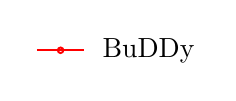
\begin{tikzpicture}
      \begin{customlegend}[
        legend columns=-1,
        legend style={draw=none,column sep=1ex},
        legend entries={BuDDy}
        ]
        \addlegendimage{style=plot_buddy}
      \end{customlegend}
    \end{tikzpicture}
    
    \caption{Minimal running time for the \emph{Queens} problems.}
  \end{figure}

\end{frame}

\begin{frame}
  \begin{figure}
    \centering
    
    \begin{tikzpicture}
      \begin{axis}[%
        width=0.73\linewidth, height=0.42\linewidth,
        every tick label/.append style={font=\scriptsize},
        % x-axis
        xlabel={number of BDD nodes},
        xmajorgrids=true,
        xmin=800000 ,
        xmax=1200000000,
        xmode = log,
        % y-axis
        ymin=2,
        ymax=5.95,
        ylabel={misses / BDD node},
        ytick distance={1},
        yminorgrids=false,
        ymajorgrids=true,
        grid style={dashed,black!20},
        ]

        \addplot [style=plot_buddy]
        table {./data/cache_buddy_misses_per_node.tex};
      \end{axis}
    \end{tikzpicture}

    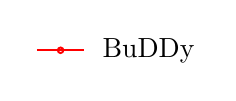
\begin{tikzpicture}
      \begin{customlegend}[
        legend columns=-1,
        legend style={draw=none,column sep=1ex},
        legend entries={BuDDy}
        ]
        \addlegendimage{style=plot_buddy}
      \end{customlegend}
    \end{tikzpicture}
    
    \caption{Cache-misses for the \emph{Queens} problems.}
  \end{figure}

\end{frame}

\blankframe

\begin{frame}
  \begin{columns}
  \begin{column}{0.49\textwidth}

    \begin{figure}
      \centering

      \begin{subfigure}{1\linewidth}
        \centering

        \begin{tikzpicture}[scale=0.9, every node/.style={transform shape}]
          % nodes
          \node[shape = circle, draw = black]
          (0) {\tiny $(0,0)$};

          \node[shape = circle, draw = black, below right= .3cm and .5cm of 0]
          (1) {\tiny $(1,0)$};

          \node[shape = circle, draw = black, below left=.3cm and .5cm of 1]
          (2) {\tiny $(2,0)$};

          \node[shape = circle, draw = black, below left=.3cm and .5cm of 2]
          (31) {\tiny $(3,0)$};
          \node[shape = circle, draw = black, below right=.3cm and .5cm of 2]
          (32) {\tiny $(3,1)$};

          % leafs
          \node[shape = rectangle, draw = black, below=.4cm of 31]
          (sink_T) {$\top$};

          \node[shape = rectangle, draw = black, below=.4cm of 32]
          (sink_F) {$\bot$};

          % arcs
          \draw[->,dashed]
          (0) edge (2)
          (1) edge (2)
          (2) edge (31)
          (31) edge (sink_T)
          (32) edge (sink_F)
          ;

          \draw[->]
          (0) edge (1)
          (1) edge (32)
          (2) edge (32)
          (31) edge (sink_F)
          (32) edge (sink_T)
          ;

          % animations
          \onslide<3-5>{ % 0
            \node[shape = circle, orange, draw = orange]
            {\tiny $(0,0)$};
            \draw[->,dashed,orange] (0) edge (2);
            \draw[->,orange] (0) edge (1);
          }

          \onslide<6-9>{ % 1
            \node[shape = circle, orange, draw = orange, below right= .3cm and .5cm of 0]
            {\tiny $(1,0)$};
            \draw[->,dashed,orange] (1) edge (2);
            \draw[->,orange] (1) edge (32);
          }

          \onslide<10-14>{ % 2
            \node[shape = circle, orange, draw = orange, below left=.3cm and .5cm of 1]
            {\tiny $(2,0)$};
            \draw[->,dashed,orange] (2) edge (31);
            \draw[->,orange] (2) edge (32);
          }

          \onslide<15-18>{ % 31
            \node[shape = circle, orange, draw = orange, below left=.3cm and .5cm of 2]
            {\tiny $(3,0)$};
            \draw[->,dashed,orange] (31) edge (sink_T);
            \draw[->,orange] (31) edge (sink_F);
          }

          \onslide<19-22>{ % 32
            \node[shape = circle, orange, draw = orange, below right=.3cm and .5cm of 2]
            {\tiny $(3,1)$};
            \draw[->,dashed,orange] (32) edge (sink_F);
            \draw[->,orange] (32) edge (sink_T);
          }
        \end{tikzpicture}

        \caption{\small $(x_0 \wedge x_1 \wedge x_3) \vee (x_2 \oplus x_3)$}
      \end{subfigure}

      %\caption{In-order traversal of BDD}
    \end{figure}

  \end{column}
  \begin{column}{0.49\textwidth}
    \centering

    \onslide<5->{ \small
      \begin{tabular}{c c c}
        \onslide<5-22>{\hspace{10pt}Seek\hspace{10pt}}
        \onslide<5-22>{& \hspace{10pt}Sum\hspace{10pt}}
        \onslide<5-23>{& \hspace{10pt}Result\hspace{10pt}}
        \\
        \textcolor{orange}{%
        \only<5-8>{$(1,0)$}%
        \only<9-13>{$(2,0)$}%
        \only<14-17>{$(3,0)$}%
        \only<18-22>{$(3,1)$}%
        }
        &
        % (1,0)
          \only<5-6>{$0$}%
          \only<7-8>{$1$}%
          % (2,0)
          \only<9-10>{$0$}%
          \only<11>{$1$}%
          \only<12-13>{$2$}%
          % (3,0)
          \only<14-15>{$0$}%
          \only<16-17>{$2$}%
          % (3,1)
          \only<18-19>{$0$}%
          \only<20>{$1$}%
          \only<21-22>{$3$}%
        &
          \only<1-16>{$0$}%
          \only<17-21>{$2$}%
          \only<22-23>{$5$}%
      \end{tabular}
    }

    \vspace{20pt}

    \onslide<2->{
      {\footnotesize Priority Queue: $Q_{\mathit{count}}$:

        \begin{tabular}{rll}
          [ & \onslide<4-6>{$(\arc{(0,0)}{\top}{(1,0)}, \quad 1)$  & ,}
          \\
            & \onslide<4-10>{$(\arc{(0,0)}{\bot}{(2,0)}, \quad 1)$  & ,}
          \\
            & \onslide<8-11>{$(\arc{(1,0)}{\bot}{(2,0)}, \quad 1)$  & ,}
          \\
            & \onslide<13-15>{$(\arc{(2,0)}{\bot}{(3,0)}, \quad 2)$  & ,}
          \\
            & \onslide<8-19>{$(\arc{(1,0)}{\top}{(3,1)}, \quad 1)$   & ,}
          \\
            & \onslide<13-20>{$(\arc{(2,0)}{\top}{(3,1)}, \quad 2)$ }  & ]
        \end{tabular}
      }
    }

  \end{column}
\end{columns}

\end{frame}

\begin{frame}[plain,noframenumbering]{} % \blankframe until reveal
  \pause

  \begin{center}
    \vspace{8pt}

    {\Huge \textbf{Adiar}}

    \vspace{12pt}

    \textcolor{gray}{\small
      \href{http://github.com/ssoelvsten/adiar}{github.com/ssoelvsten/adiar}
    }
  \end{center}
\end{frame}

\begin{frame}
  \begin{figure}
    \centering
    
    \begin{tikzpicture}
      \begin{axis}[%
        width=0.70\linewidth, height=0.42\linewidth,
        every tick label/.append style={font=\scriptsize},
        % x-axis
        xlabel={number of BDD nodes},
        xmajorgrids=true,
        xmin=51000000,
        xmax=300000000000,
        xmode = log,
        % y-axis
        ymin=0,
        ymax=2.2,
        ytick distance={0.5},
        ylabel={$\mu$s / BDD node},
        yminorgrids=true,
        ymajorgrids=true,
        grid style={dashed,black!20},
        ]     
        
        \only<2-> {
          \addplot+ [style=plot_cudd]
          table {./data/queens_cudd_time_per_node.tex};
        }

        \only<3-> {
          \addplot+ [style=plot_sylvan]
          table {./data/queens_sylvan_time_per_node.tex};
        }
        
        \only<4-> {
          \addplot+ [style=plot_adiar]
          table {./data/queens_adiar_time_per_node.tex};
        }
      \end{axis}

    \end{tikzpicture}

    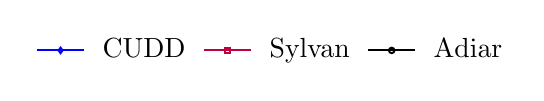
\begin{tikzpicture}
      \begin{customlegend}[
        legend columns=-1,
        legend style={draw=none,column sep=1ex},
        legend entries={CUDD, Sylvan, Adiar}
        ]
        \addlegendimage{style=plot_cudd}
        \addlegendimage{style=plot_sylvan}
        \addlegendimage{style=plot_adiar}
      \end{customlegend}
    \end{tikzpicture}
    
    \caption{Minimal running time for the \emph{Queens} problems.}
  \end{figure}
\end{frame}

\blankframe

\begin{frame}

  \begin{table}
    \centering
    \begin{tabular}{r | l}
      Algorithm                         & Time (s)
      \\ \hline
      $f \leftrightarrow g \equiv \top$ & 0.38
      \\ \onslide<2->{
      $O(N \log N)$                     & 0.058}
      \\ \onslide<3->{
      $O(N)$                            & 0.006}
    \end{tabular}

    \caption{Checking the (EPFL Benchmark) \emph{voter} circuit's single output
      gate ($\abs{N_f} = \abs{N_g} = 5.76~\text{MiB}$).}
  \end{table}

\end{frame}

\blankframe

\begin{frame}[plain,noframenumbering]
  {\Large \textbf{Steffan Christ Sølvsten}}
  \vspace{1pt} {\hrule width0.45\linewidth}

  \vspace{5pt}

  \begin{itemize}
  \item[\faIcon{envelope}] \mailto{soelvsten@cs.au.dk}
  \item[\faIcon{twitter}] \href{https://www.twitter.com/ssoelvsten}{@ssoelvsten}
  \end{itemize}

  \vspace{10pt}

  {\Large \textbf{Adiar}}
  \vspace{1pt} {\hrule width0.45\linewidth}

  \vspace{5pt}

  \begin{itemize}
  \item[\faIcon{code}]
    \href{http://github.com/ssoelvsten/adiar}{github.com/ssoelvsten/adiar}
  \item[\faIcon{book}\hspace{2pt}]
    \href{http://ssoelvsten.github.io/adiar}{ssoelvsten.github.io/adiar}
  \end{itemize}


  \vspace{10pt}

  
\includegraphics[width=0.2\linewidth]{external/aulogo_uk_var2_black.eps}
\end{frame}

\end{document}

%%% Local Variables:
%%% mode: latex
%%% TeX-master: t
%%% End:
